\chapter{วิธีการดำเนินงาน}
\centering{\bf{\textit{(ตัวอย่างเนื้อหาบทที่สาม...)}}} \\
\thaijustify{
    ในบทที่ 3 จะกล่าวถึงภาพรวม... โครงสร้างระบบ... ที่วางแผนและออกแบบเอาไว้
}
\section{รายละเอียดของโครงงาน}
    \thaijustify{
        ในหัวข้อแรกของบทที่ 3 กลุ่มเราจะ...
    }
    \subsection{ข้อกำหนดและความต้องการของระบบ}
        \thaijustify{
            ในส่วนนี้ จะกล่าวถึงข้อกำหนดของซอฟต์แวร์หรือ User Requirements...
        }
        \begin{longtable}{p{3cm}|ccccccc}
            % First header
                \caption{ข้อกำหนดของซอฟต์แวร์}\label{tbl:soft-req1} \\ % First caption
                \hline\hline
                Feature & Guest User & Registered User &  Student & Attendee & Moderator & Owner & Admin \\ 
                \hline\hline
            \endfirsthead
            % Re-occurring header
                \caption[]{ข้อกำหนดของซอฟต์แวร์ (ต่อ)} \\ % Cont. caption
                \hline\hline
                Feature & Guest User & Registered User &  Student & Attendee & Moderator & Owner & Admin \\ 
                \hline\hline
            \endhead
            % First footer
                \hline \hline
            \endfoot
            % Last footer
                \hline \hline
            \endlastfoot
            % Body
            เข้าสู่ระบบ & \checkmark & \checkmark & \checkmark & \checkmark & \checkmark & \checkmark & \checkmark \\ \hline
            ออกจากระบบ & & \checkmark & \checkmark & \checkmark & \checkmark & \checkmark & \checkmark \\ \hline
            กู้รหัสผ่าน & \checkmark & \checkmark & \checkmark & \checkmark & \checkmark & \checkmark & \checkmark \\ \hline
            ดูข้อมูลส่วนตัว  & & \checkmark & \checkmark & \checkmark & \checkmark & \checkmark & \checkmark \\ \hline
            ...  & & & & & & & \checkmark \\ \hline
            ...  & & & & & & & \checkmark \\ \hline
            ...  & & & & & & & \checkmark \\ \hline
            ...  & & & & & & & \checkmark \\ \hline
            ...  & & & & & & & \checkmark \\ \hline
            ...  & & & & & & & \checkmark \\ \hline
            ...  & & & & & & & \checkmark \\ \hline
            ...  & & & & & & & \checkmark \\ \hline
            ...  & & & & & & & \checkmark \\ \hline
            ...  & & & & & & & \checkmark \\ \hline
            ...  & & & & & & & \checkmark \\ \hline
            ...  & & & & & & & \checkmark \\ \hline
            ...  & & & & & & & \checkmark \\ \hline
            ...  & & & & & & & \checkmark \\ \hline
            ...  & & & & & & & \checkmark \\ \hline
            ...  & & & & & & & \checkmark \\ \hline
            ...  & & & & & & & \checkmark \\ \hline
            ...  & & & & & & & \checkmark \\ \hline
            ...  & & & & & & & \checkmark \\ \hline
            ...  & & & & & & & \checkmark \\ \hline
            ...  & & & & & & & \checkmark \\ \hline
            ...  & & & & & & & \checkmark \\ \hline
            ...  & & & & & & & \checkmark \\ \hline
            ...  & & & & & & & \checkmark \\ \hline
            ...  & & & & & & & \checkmark \\ \hline
            ...  & & & & & & & \checkmark \\ \hline
            ...  & & & & & & & \checkmark \\ \hline
            ...  & & & & & & & \checkmark \\ \hline
            ...  & & & & & & & \checkmark \\ \hline
            ...  & & & & & & & \checkmark \\ \hline
            ...  & & & & & & & \checkmark \\ \hline
            ...  & & & & & & & \checkmark \\ \hline
            ...  & & & & & & & \checkmark \\ \hline
            ...  & & & & & & & \checkmark \\ \hline
            ...  & & & & & & & \checkmark \\ \hline
        \end{longtable}
        \pagebreak
    \subsection{กรณีการใช้งาน}
        \thaijustify{
            ในส่วนนี้ทางคณะผู้จัดทำได้นำเอาข้อมูลข้อกำหนดและข้อใช้งานต่าง ๆ ที่ได้เก็บรวบรวม พร้อมข้อมูลประเภทผู้ใช้ทั้งหมดรวมไปถึงข้อใช้งานที่ผู้ใช้แต่ละประเภทเข้าถึงได้ในหัวข้อที่แล้ว  (จาก\cref{tbl:soft-req1}) มาวาดเป็นแผนผังกรณีใช้งานใน\cref{fig:usecase} เพื่อให้ผู้อ่านดูแล้วเข้าใจง่ายขึ้น
        } 
        \begin{figure}[!h]
        \centering
            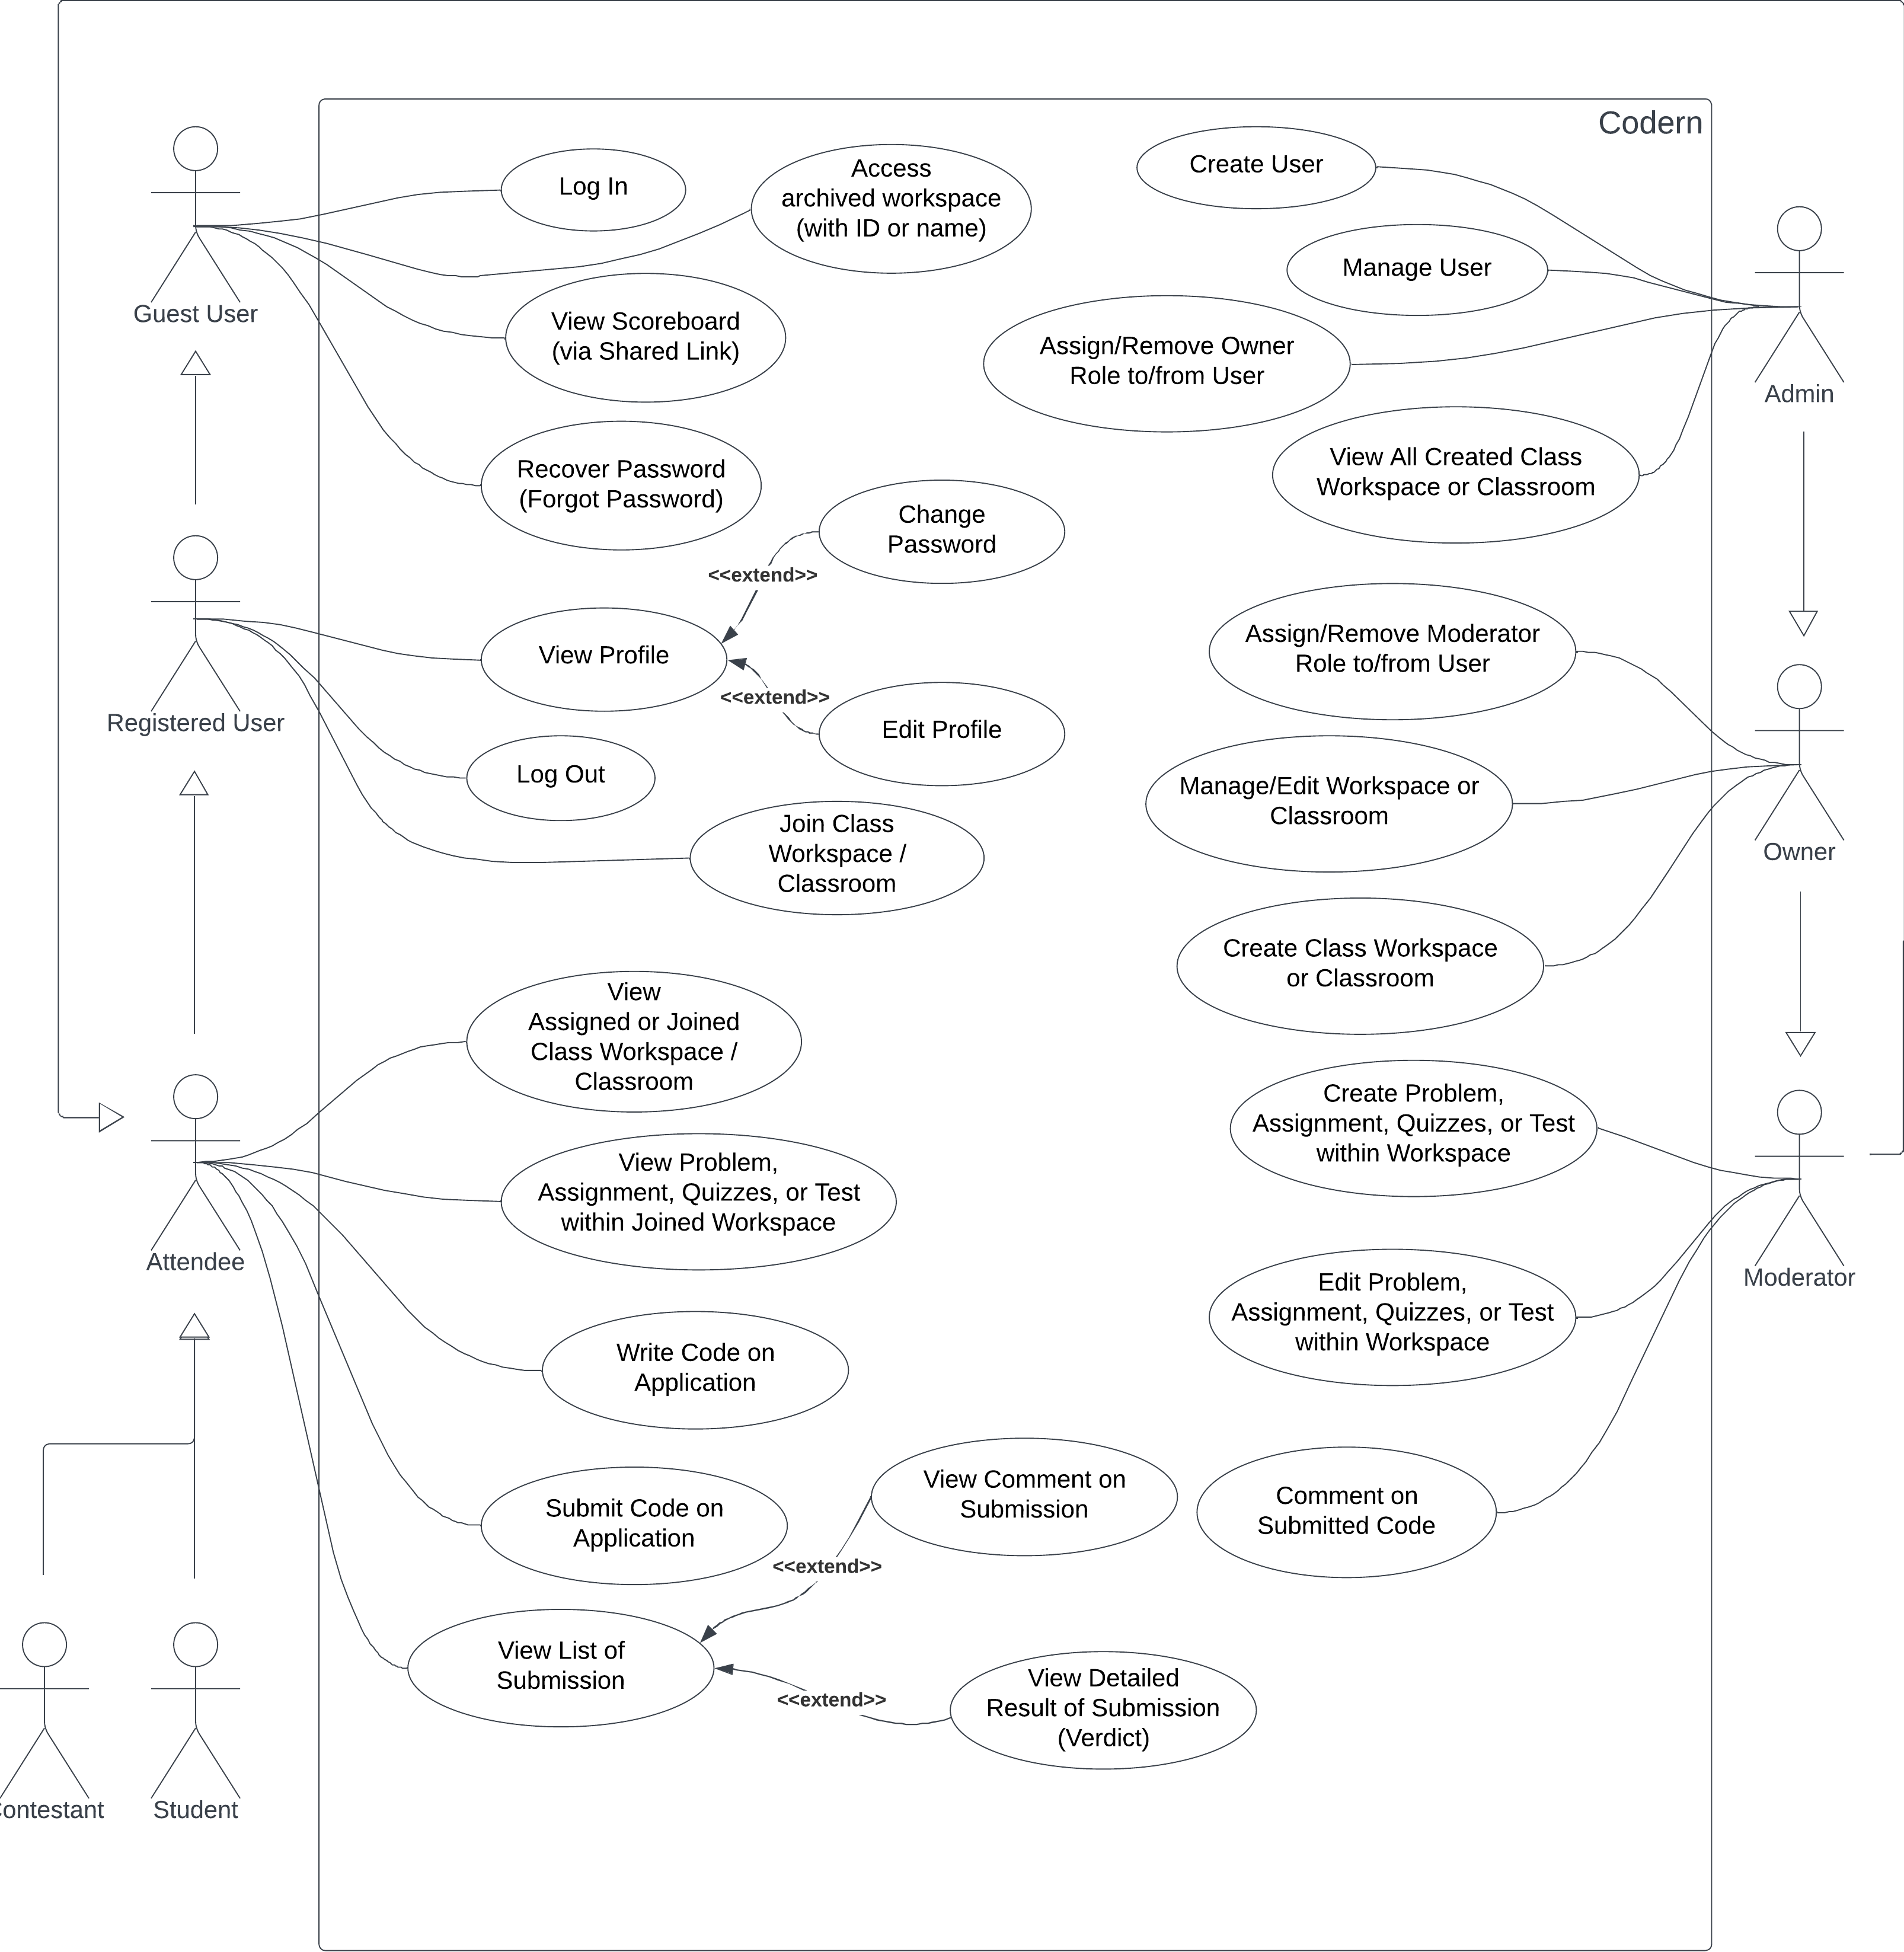
\includegraphics[width=15cm]{chapters/3/figures/design/usecase-v5.png}
        \caption[ภาพเเผนผังกรณีใช้งาน]{ภาพเเผนผังกรณีใช้งาน วาดด้วย \href{https://lucid.app/}{LucidChart}}
        \label{fig:usecase}
        \end{figure}
        \pagebreak
    \subsection{คำบรรยายแผนผังกรณีใช้งาน}
        \thaijustify{
            จาก\cref{fig:usecase} ในหัวข้อที่แล้ว เป็น... ในโครงงานซอฟต์แวร์นี้ได้แบ่งประเภทผู้ใช้ออกเป็น ?? ประเภท ได้แก่...
        }
        \subsubsection{Guest User (บุคคลทั่วไป)}
            \thaijustify{
                บุคคลทั่วไป สามารถเข้าใช้งาน feature พื้นฐานของซอฟต์แวร์ได้ดังนี้
            }
            \begin{enumerate}
                \item “Log In” คือ การล็อกอินเข้าสู่ระบบ
                \item “View Scoreboard (via Shared Link)” คือ การเข้าถึงตารางคะแนนด้วยลิงก์ที่ถูกแชร์มา
                \item “Recover Password” คือ การกู้คืนรหัสผ่าน กรณีที่หลงลืมหรือสูญหาย
            \end{enumerate}
        \subsubsection{Registered User (ผู้ใช้ทั่วไป)}
            \thaijustify{
                ผู้ใช้ทั่วไปก็คือบุคคลทั่วไปที่มีบัญชีในระบบ (Admin อาจได้สร้างไว้ให้ หรือไม่ก็สมัครเอง) โดยผู้ใช้ทั่วไปสามารถเข้าถึง feature พื้นฐานของซอฟต์แวร์ได้เหมือนกับบุคคลทั่วไป (Guest User) และยังสามารถเข้าใช้ feature เพิ่มเติมได้ดังต่อไปนี้...
            }
    \pagebreak
\section{สถาปัตยกรรมระบบ}
    \thaijustify{
        ...
    }
    \pagebreak
\section{ส่วนประสานต่อผู้ใช้}
    \thaijustify{
        สำหรับในส่วนหน้าประสานงานผู้ใช้หรือ User Interface (UI) ... ได้ออกแบบไว้ทั้งหมดดังนี้...
    }
    \begin{figure}[H]
    \centering
        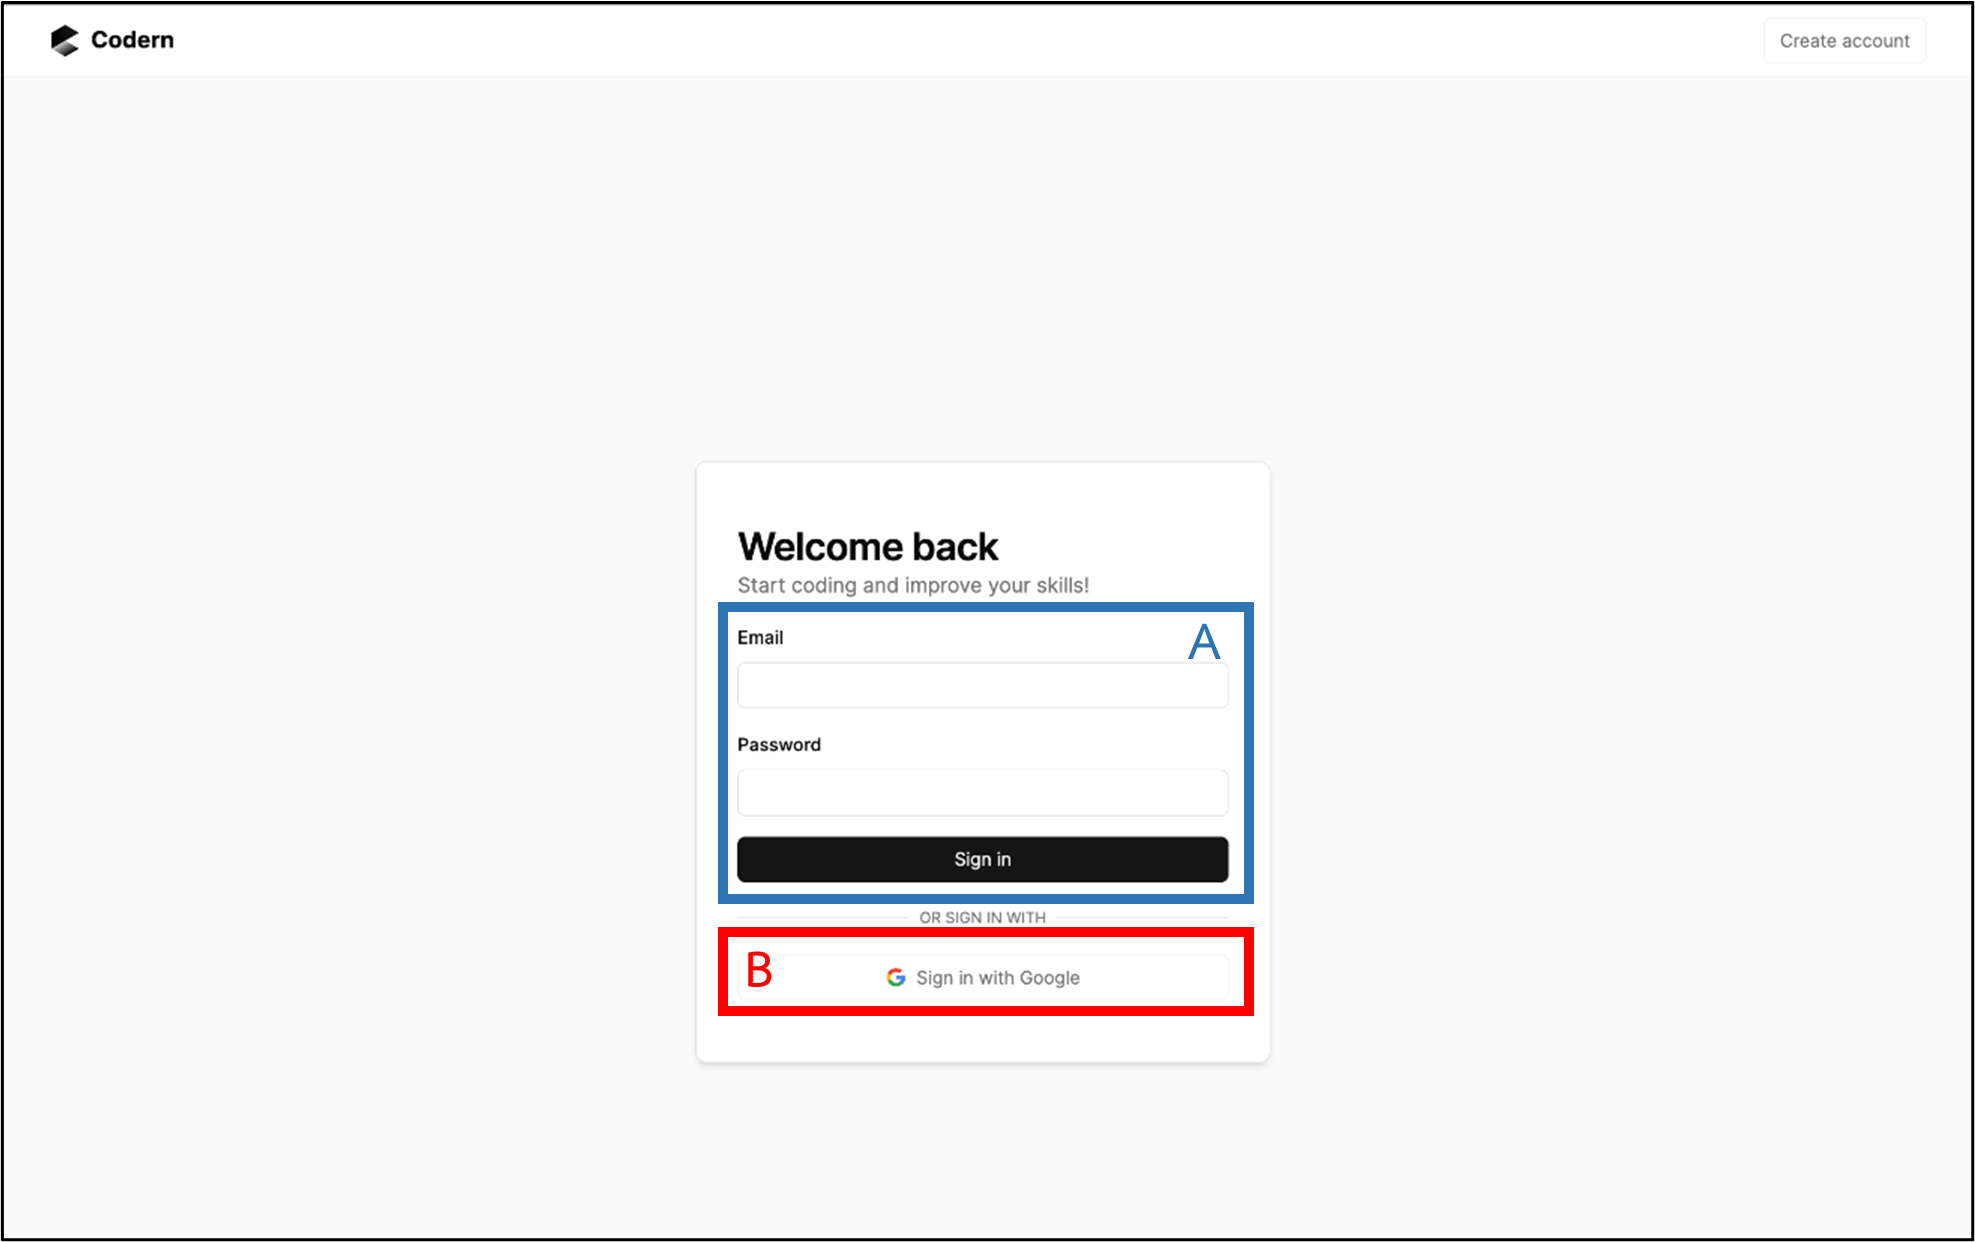
\includegraphics[width=15cm]{chapters/3/figures/ui/ui-login1.png}
        \caption[ส่วนประสานต่อผู้ใช้ หน้าเข้าสู่ระบบ]{ส่วนประสานต่อผู้ใช้ หน้าเข้าสู่ระบบ}
        \label{fig:ui-login}
    \end{figure}
    \thaijustify{
        ใน\cref{fig:ui-login} เป็นหน้าสำหรับล็อกอินเข้าระบบใช้งานทั้งหมดของซอฟต์แวร์ โดยสามารถเลือกล็อกอินได้สองวิธี; ด้วยอีเมลเเละรหัสผ่าน (กรอบสีน้ำเงิน A) และล็อกอินผ่านกูเกิ้ล (กรอบสีแดง B)...
    }  
\pagebreak
\section{โครงสร้างฐานข้อมูล}
    \thaijustify{
       ...
    }
    \pagebreak
    \subsection{คำบรรยายโครงสร้างฐานข้อมูล}
    \thaijustify{
        ในส่วนนี้ทางกลุ่มเราจะอธิบาย รายละเอียด... จากฐานข้อมูลในส่วนที่แล้ว...
    }
    \begin{enumerate}
        %% User's Relations
        \item \textbf{User}
            เป็นตารางที่เก็บข้อมูลของผู้ใช้แต่ละคน เช่นอีเมลล์, ชื่อ-นามสกุลขของผู้ใช้ เป็นต้น จากความสัมพันธ์ของตารางดังกล่าว กับตารางอื่น ๆ สามารถสรุปความสัมพันธ์ได้ดังนี้
            \begin{figure}[H]
                \centering
                \subfloat[แผนผังแสดงความสัมพันธ์ระหว่างตาราง User และ Session]{
                    \begin{tikzpicture}[auto,node distance=0.7cm]
                        % First Entity
                        \node[entity] (node1) {User};
                        % [grow=up,sibling distance=3cm]
                        % child {node[attribute] {Attribute 1}}
                        % child {node[attribute] {Attribute 2}}
                        % child[grow=left,level distance=3cm] {node[attribute] {Attribute 3}};
                        % Relationship
                        \node[relationship] (rel1) [right = of node1] {has};
                        % Second Entity
                        \node[entity] (node2) [right = of rel1]	{Session};
                        % Draw an edge between rel1 and node1; rel1 and node2
                        \path (rel1) edge node {\(1\)-\(1\)} 
                        (node1) edge node {\(1\)-\(m\)}	(node2);
                    \end{tikzpicture}
                    \label{fig:db-user-session}
                } \hspace{0.5cm}
                \subfloat[แผนผังแสดงความสัมพันธ์ระหว่างตาราง User และ Workspace]{
                    \begin{tikzpicture}[auto,node distance=0.7cm]
                        % First Entity
                        \node[entity] (node1) {User};
                        % Relationship
                        \node[relationship] (rel1) [right = of node1] {owns};
                        % Second Entity
                        \node[entity] (node2) [right = of rel1]	{Workspace};
                        % Draw an edge between rel1 and node1; rel1 and node2
                        \path (rel1) edge node {\(1\)-\(1\)} 
                        (node1) edge node {\(0\)-\(m\)}	(node2);
                    \end{tikzpicture}
                    \label{fig:db-user-workspace}
                } \\
                \subfloat[แผนผังแสดงความสัมพันธ์ระหว่างตาราง User และ WorkspaceParticipant]{
                    \begin{tikzpicture}[auto,node distance=0.7cm,]
                        % First Entity
                        \node[entity] (node1) {User};
                        % Relationship
                        \node[relationship] (rel1) [right = of node1] {becomes};
                        % Second Entity
                        \node[entity] (node2) [right = of rel1]	{WorkspaceParticipant};
                        % Draw an edge between rel1 and node1; rel1 and node2
                        \path (rel1) edge node {\(1\)-\(1\)} 
                        (node1) edge node {\(0\)-\(m\)}	(node2);
                    \end{tikzpicture}
                    \label{fig:db-user-workspace_participant}
                } \\
                \subfloat[แผนผังแสดงความสัมพันธ์ระหว่างตาราง User และ Submission]{
                    \begin{tikzpicture}[auto,node distance=0.7cm]
                        % First Entity
                        \node[entity] (node1) {User};
                        % Relationship
                        \node[relationship] (rel1) [right = of node1] {submit};
                        % Second Entity
                        \node[entity] (node2) [right = of rel1]	{Submission};
                        % Draw an edge between rel1 and node1; rel1 and node2
                        \path (rel1) edge node {\(1\)-\(1\)} 
                        (node1) edge node {\(0\)-\(m\)}	(node2);
                    \end{tikzpicture}
                    \label{fig:db-user-submission}
                }
                \caption[กลุ่มแผนผังแสดงความสัมพันธ์ของตาราง User]{กลุ่มแผนผังแสดงความสัมพันธ์ของตาราง User}
                \label{fig:db-user}
            \end{figure}
            \begin{itemize}
                \item จากรูปที่~\ref{fig:db-user-session} ผู้ใช้สามารถที่จะเข้าสู่ระบบได้หลายเครื่องพร้อม ๆ กัน ก็คือผู้ใช้เข้าสู่ระบบได้ (has) หลาย Session พร้อมกัน
                \item จากรูปที่~\ref{fig:db-user-workspace} ผู้ใช้สามารถที่จะครอบครอง (owns) Workspace ได้มากกว่า 1 Workspace
                \item จากความสัมพันธ์ในรูป~\ref{fig:db-user-workspace_participant} ผู้ใช้สามารถที่จะเป็นคนเข้าร่วม (join workspace) ในกลุ่มเรียนหรือห้องเรียน (หรือ Workspace Participant) ได้มากกว่า 1 ห้องเรียนหรือกลุ่มเรียน หรือ Workspace
                \item จากรูปที่~\ref{fig:db-user-submission} ผู้ใช้สามารถที่จะส่ง (submit) ได้มากกว่า 1 ห้องเรียนหรือกลุ่มเรียน หรือ Workspace
            \end{itemize}
        %% Session's Relations
        \item \textbf{Session}
            เป็นตารางที่จะเก็บข้อมูล Session หรือข้อมูลเครื่อง ข้อมูลช่องทางที่ผู้ใช้เข้าสู่ระบบ สามารถสรุปความสัมพันธ์ได้ดังนี้
            \begin{itemize}
                \item ถึงเเม้ผู้ใช้หนึ่งท่านสามารถที่จะมีได้หลาย Session คือผู้ใช้สามารถเข้าสู่ระบบได้หลายเครื่องพร้อมก่อน แต่ Session เป็นของผู้ใช้แค่คนเดียวเท่านั้นตามรูปที่~\ref{fig:db-user-session}
            \end{itemize}
        %% Workspace's Relations
        \item \textbf{Workspace}
            เป็นตารางที่สร้างขึ้นมาเก็บข้อมูลห้องเรียนหรือกลุ่มเรียน (Workspace) มีความสัมพันธ์กับตารางอื่นดังต่อไปนี้...
   \end{enumerate} 
    \subsection{พจนานุกรมข้อมูล}
        \thaijustify{
            ในส่วนนี้ จะเป็นพจนานุกรม... ที่อยู่ในแผนภาพฐานข้อมูลในหัวข้อก่อน   
        }
        \begin{table}[H]
            \centering
            \caption{พจนานุกรมข้อมูลของตาราง User}\label{tbl:data-dict-user}
            \begin{tabular}{p{2cm}|p{4cm}p{2cm}p{3cm}p{2cm}} \hline\hline
                Attribute Name & Description & Data Type & Constraints & References \\ \hline\hline
                id & รหัส ID การส่งงาน & bigint & Primary Key & - \\
                a\_id & ID ของโจทย์ & bigint & Foreign Key, Not Null & Assign \\
                uid & ID ของผู้ใช้ & varchar(64) & Foreign Key, Not Null & User \\
                ... & ... & varchar(128) & Not Null & - \\
                ... & ... & longtext & - & - \\ \hline\hline
            \end{tabular}   
        \end{table}
    \pagebreak
\section{แผนผัง UML}
    \thaijustify{
        สำหรับในส่วนนี้ จะแสดงและบรรยาย... เเผนผัง UML ที่ได้วาดมา...
    }
\pagebreak